% \textbf{Эксперимент по MBL}.
Рассмотрим экспериментальную реализацию системы \eqref{9:model} в \cite{Choi_2016}. Для этого, совместив лазерные лучи, получим некоторую интерференционную картину, пучности которой при красной отстройке будут выступать минимуми потенциала для атомов в силу их поляризуемости (альтернативой может выступат решётка optical tweezers). Между этими минимумами потенциала атомы будет туннелировать с характерной энергией $J$, которую и будем использовать в качестве масштаба по энергиям.  Подстроить взаимодействие $U$ между атомами можем с помощью резонансов Фейшбаха, выкрутив которое до значения $U=24J$ получим систему близкую к hard-bosons. Поверх решётки наложим глобальный гармонический потенциал, также фокусировкой лазера. Заполним ловушку достаточно холодными атомами, с помощью микроволнового ножа оставим заполненной только левую половину и немного подождём (fig. \ref{fig:loc2D1}). Шумы $\Delta$ в систему добавляются с помощью DMD (альтернативно используются SLM, AOD или квазслучайный потенциал как в \cite{schreiber_observation_2015}, подробнее в \cite{abanin_many-body_2019}), результат усредняют по 50 реализациям $\delta_j$.

\begin{figure}[h]
    \centering
    \addletter{80}{a}
    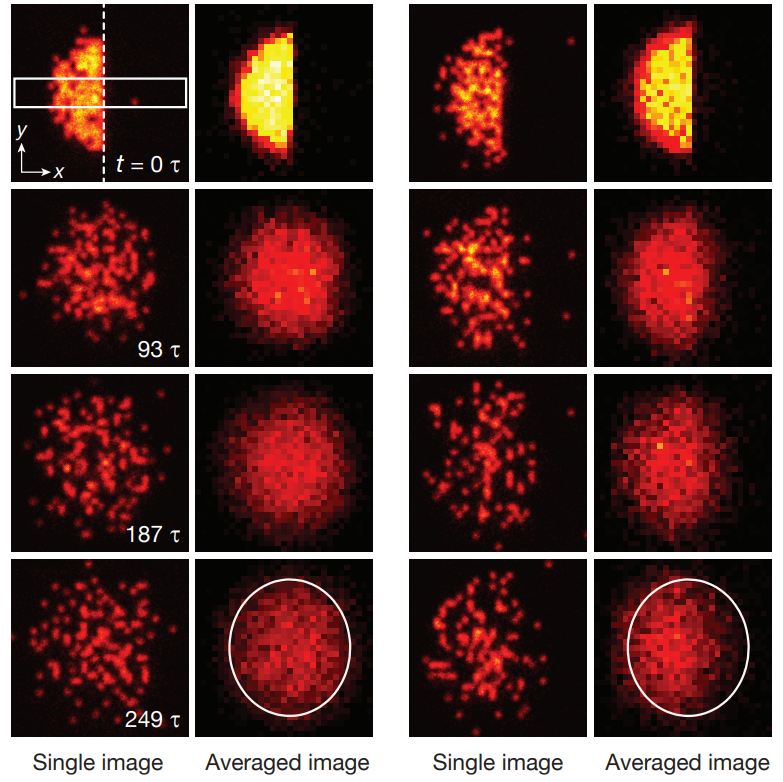
\includegraphics[align=c, width=0.33\textwidth]{imgs/MBL_2D_exp_1.png}
    \hspace{10 mm} 
    \addletter{80}{b}
    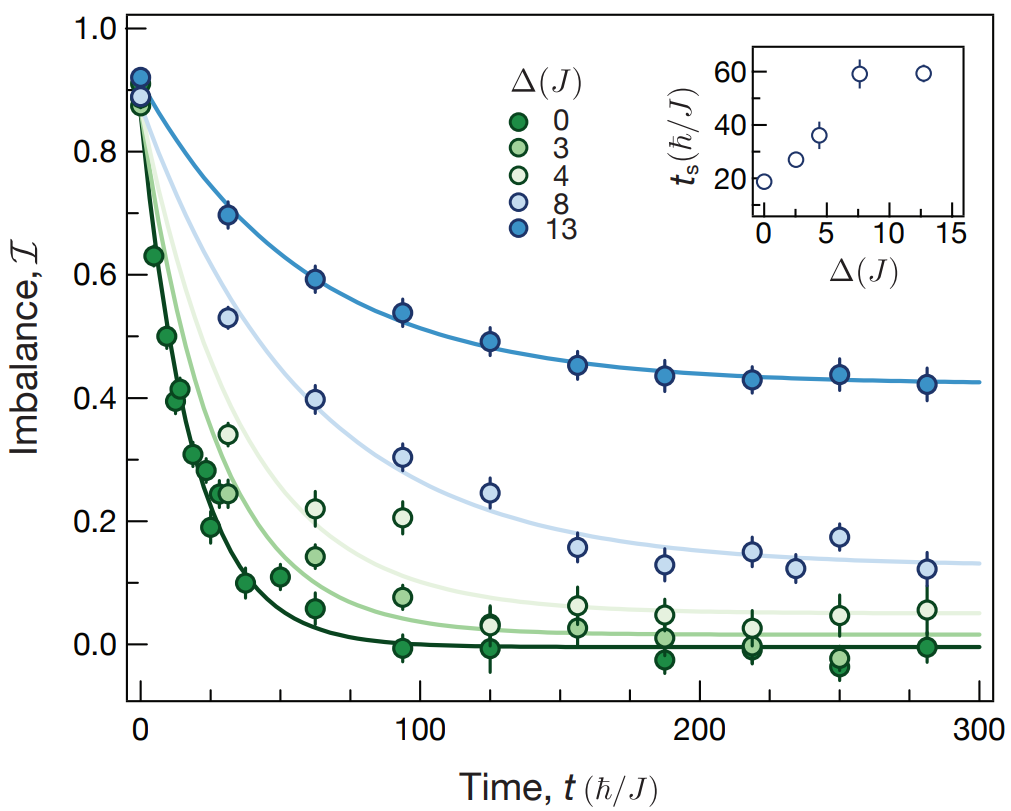
\includegraphics[align=c, width=0.4\textwidth]{imgs/MBL_2D_exp_2.png}
    % 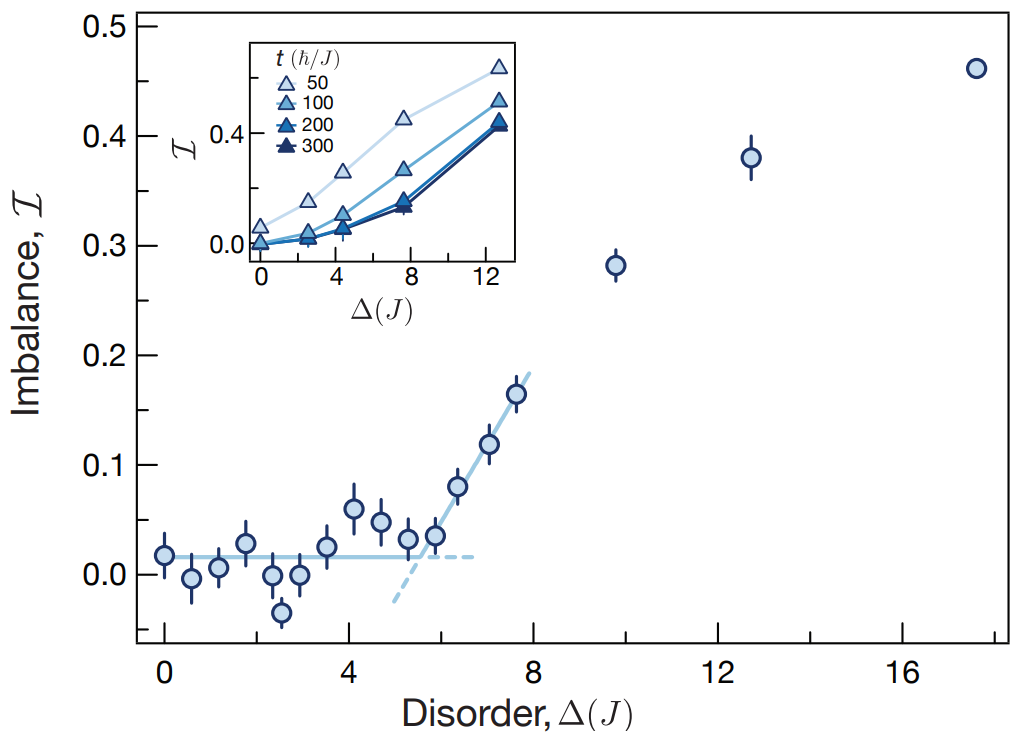
\includegraphics[align=c, width=0.4\textwidth]{imgs/MBL_2D_exp_3.png}
    \caption{
        a) Raw fluorescence images (red to yellow corresponds to increasing detected light level) showing the evolution of the initial density step without disorder \cite{Choi_2016} . 
        b) Relaxation dynamics of a density domain wall \cite{Choi_2016} .
    }
    \label{fig:loc2D1}
\end{figure}


Видно, что в отсутсвии шумов система выходит на термальное состояние -- термализация ($\mathcal{I} \to 0$). При достаточно сильных шумах наступает локализация: $\mathcal{I}(t \to \infty) = \mathcal{I}_\infty > 0$. Считая выход на $\mathcal{I}_\infty$ экспоненциальным можем заметить, как растёт необходимое для выхода на стационырное состояние по мере увеличения уровня шума. 

Видно, что $\mathcal{I}_\infty > 0$ появляется с $\sub{\Delta}{c} \approx 5.5(4) J$. В статье подчеркивают, что $\sub{\Delta}{c}$ будет увеличиваться по мере decreasind initial filling. The clear difference in critical disorder strengths highlights the strong influence of interactions on the localization.
